%!TEX root = ../main.tex
%%%%%%%%%%%%%%%%%%%%%%%%%%%%%%%%%%
% Links:
%
% Difficulty:
% Companies: 
%%%%%%%%%%%%%%%%%%%%%%%%%%%%%%%%%%


%\begin{figure}
%	\centering
%	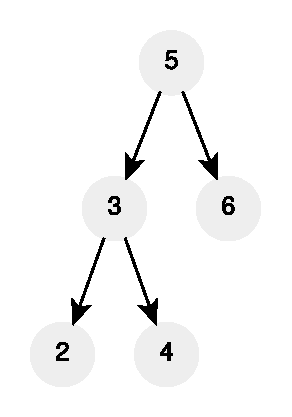
\includegraphics[width=\textwidth]{sources/kth_smallest_in_sorted_matrix/images/example1}
%	\caption[Sample short cpation]{Sample Caption}.
%	\label{fig:kth_smallest_in_sorted_matrix:example1}
%\end{figure}

\chapter{$k^{th}$ smallest element in a sorted matrix}
\label{ch:kth_smallest_in_sorted_matrix}
\section*{Introduction}

\section{Problem statement}
\begin{exercise}
\label{example:kth_smallest_in_sorted_matrix:exercice1}
Write a function that, given an square matrix $M$ of size $n$  where each of individual row and column is sorted in ascending order and an integer $1 \leq k \leq n^2$
returns the $k^{th}$ smallest element in $M$.


You can assume the elements of $M$ to be always in the range $[0,n^2]$.

	%example1
	\begin{example}
		\label{example:kth_smallest_in_sorted_matrix:example1}
		\hfill \\
		Given $M=\{\{1,5,9\},\{10,15,13\},\{12,13,15\}\}$ (as shown in Table \ref{}) and $k=8$ the function returns $13$. See table
	\end{example}
\end{exercise}
\begin{wraptable}{r}{3.5cm}
	\centering
	\begin{tabular}{|c|c|c|}
	\hline
	1  & 5  & 9  \\ \hline
	10 & 15 & 13 \\ \hline
	12 & 13 & 15 \\ \hline
	\end{tabular}%
	\caption{Tabular representation of Example \ref{example:kth_smallest_in_sorted_matrix:example1}}
	\label{tab:kth_smallest_in_sorted_matrix:example1}
\end{wraptable} 


\section{Clarification Questions}

\begin{QandA}
	\item Can we assume the input to be always valid i.e. having rows and column sorted?
	\begin{answered}
		\textit{Yes, there is no need to do input validation.}
	\end{answered}
	
	
\end{QandA}

\section{Discussion}
\label{kth_smallest_in_sorted_matrix:sec:discussion}


\subsection{Brute-force}
\label{kth_smallest_in_sorted_matrix:sec:bruteforce}

\lstinputlisting[language=c++, caption={Naive brute-force solution.},label=list:kth_smallest_in_sorted_matrix]{sources/kth_smallest_in_sorted_matrix/kth_smallest_in_sorted_matrix_solution1.cpp}

\subsection{Brute-force constant space}
\label{kth_smallest_in_sorted_matrix:sec:bruteforce_constant_space}

\lstinputlisting[language=c++, caption={Brute-force solution using constnat space.},label=list:kth_smallest_in_sorted_matrix]{sources/kth_smallest_in_sorted_matrix/kth_smallest_in_sorted_matrix_solution2.cpp}


\subsection{Binary Search}
\label{kth_smallest_in_sorted_matrix:sec:binarysearch}

\lstinputlisting[language=c++, caption={Solution using binary search.},label=list:kth_smallest_in_sorted_matrix]{sources/kth_smallest_in_sorted_matrix/kth_smallest_in_sorted_matrix_solution3.cpp}
